% !TEX root = CSC104LectureNotes.tex

\chapter{IDLE}
\label{chapter:idle}

\addindex{IDLE}{IDLE} is a simple graphical development environment for the Python programming language.  It is available for Windows, MacOS, and Linux.

IDLE provides an \textit{interactive} programming environment, as discussed in Section 1.2 of the textbook.  It also provides a way for you to run programs that were prepared earlier and saved.

\section{Using IDLE}

\subsection{Windows}

I downloaded Python from the official Python website, \url{https://www.python.org/downloads/}, and this download included IDLE.  Make sure to download the most recent available version of Python.  After running the installation program, I was able to run IDLE by pressing the Windows button in the lower left corner of the screen and then searching for IDLE.  When you initially run the program, you should see a window like the one in Figure \ref{fig:idlewin} on Page \pageref{fig:idlewin}.

\begin{myfigure}[label=fig:idlewin]{IDLE Running on Windows 10}
    \centering
    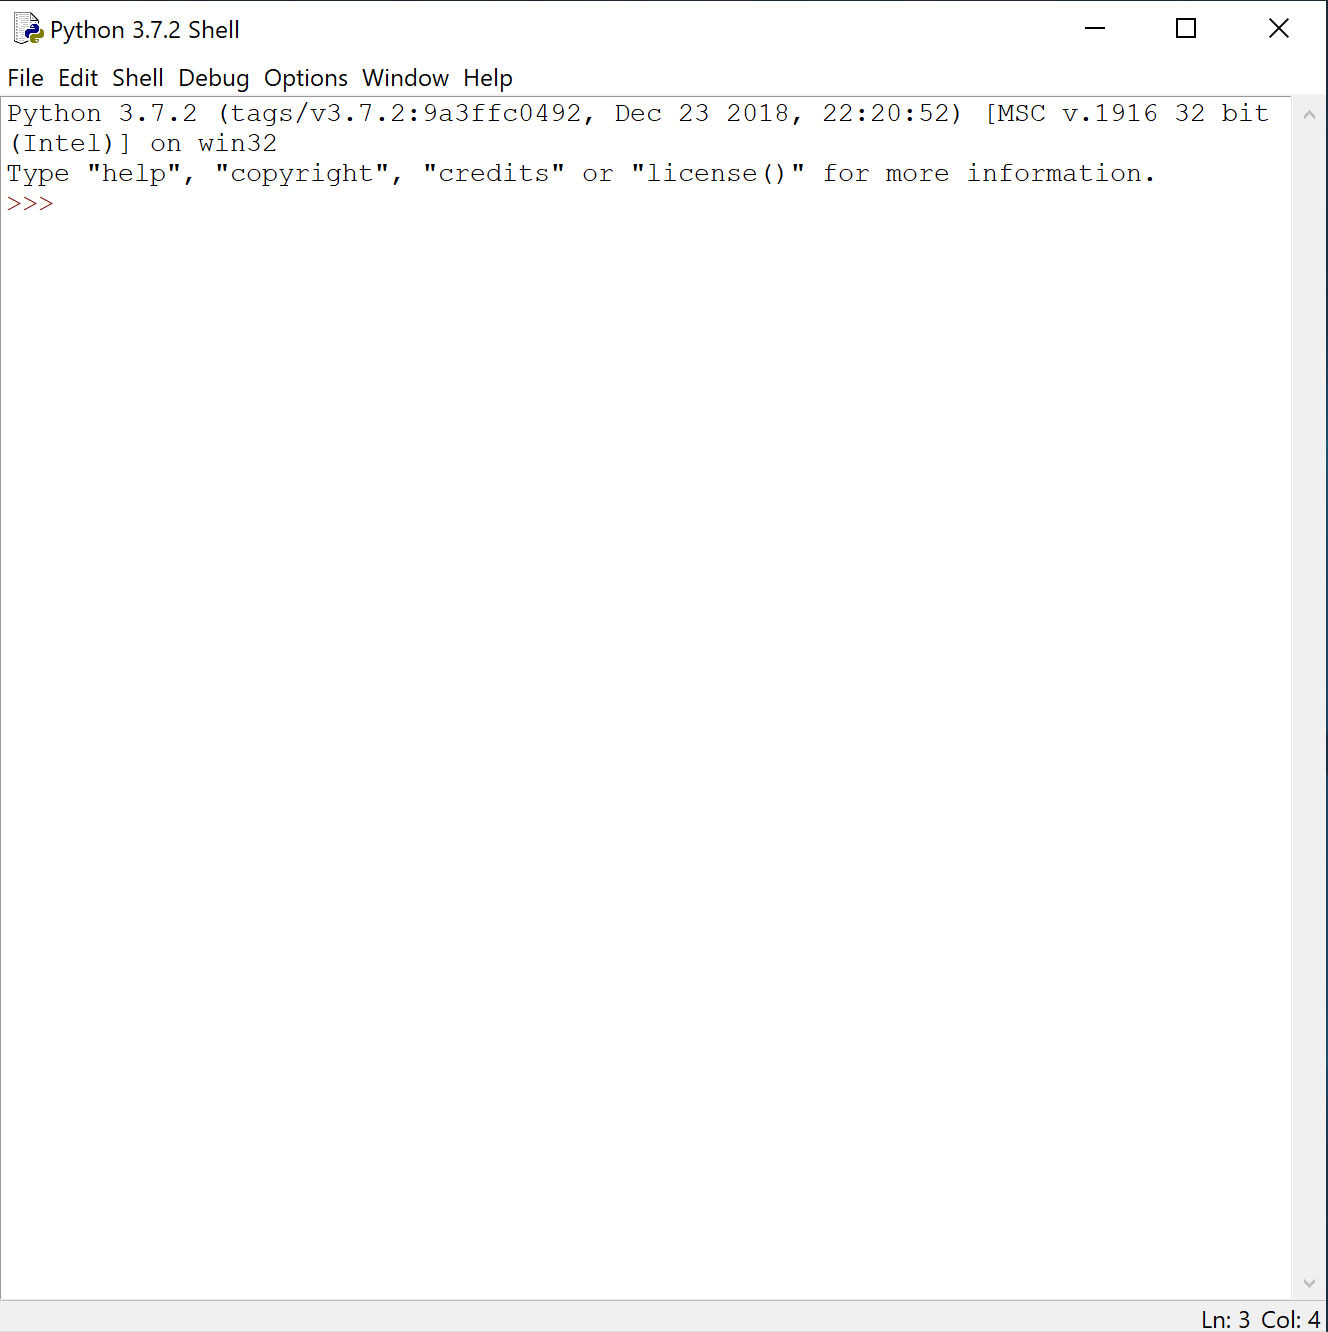
\includegraphics[scale=0.6]{screenshots/idlewin.png}
\end{myfigure}

Using the Option menu, I was able to change the font face to something nicer (I changed it to \href{Fira Code}{https://www.fontsquirrel.com/fonts/fira-code}, the same font used for code examples in these notes) and the font size to something more readable, as you see in Figure \ref{fig:idlewin-hw} on Page \pageref{fig:idlewin-hw}.

\begin{myfigure}[label=fig:idlewin-hw]{IDLE Running on Windows 10 with the Fira Code Font}
    \centering
    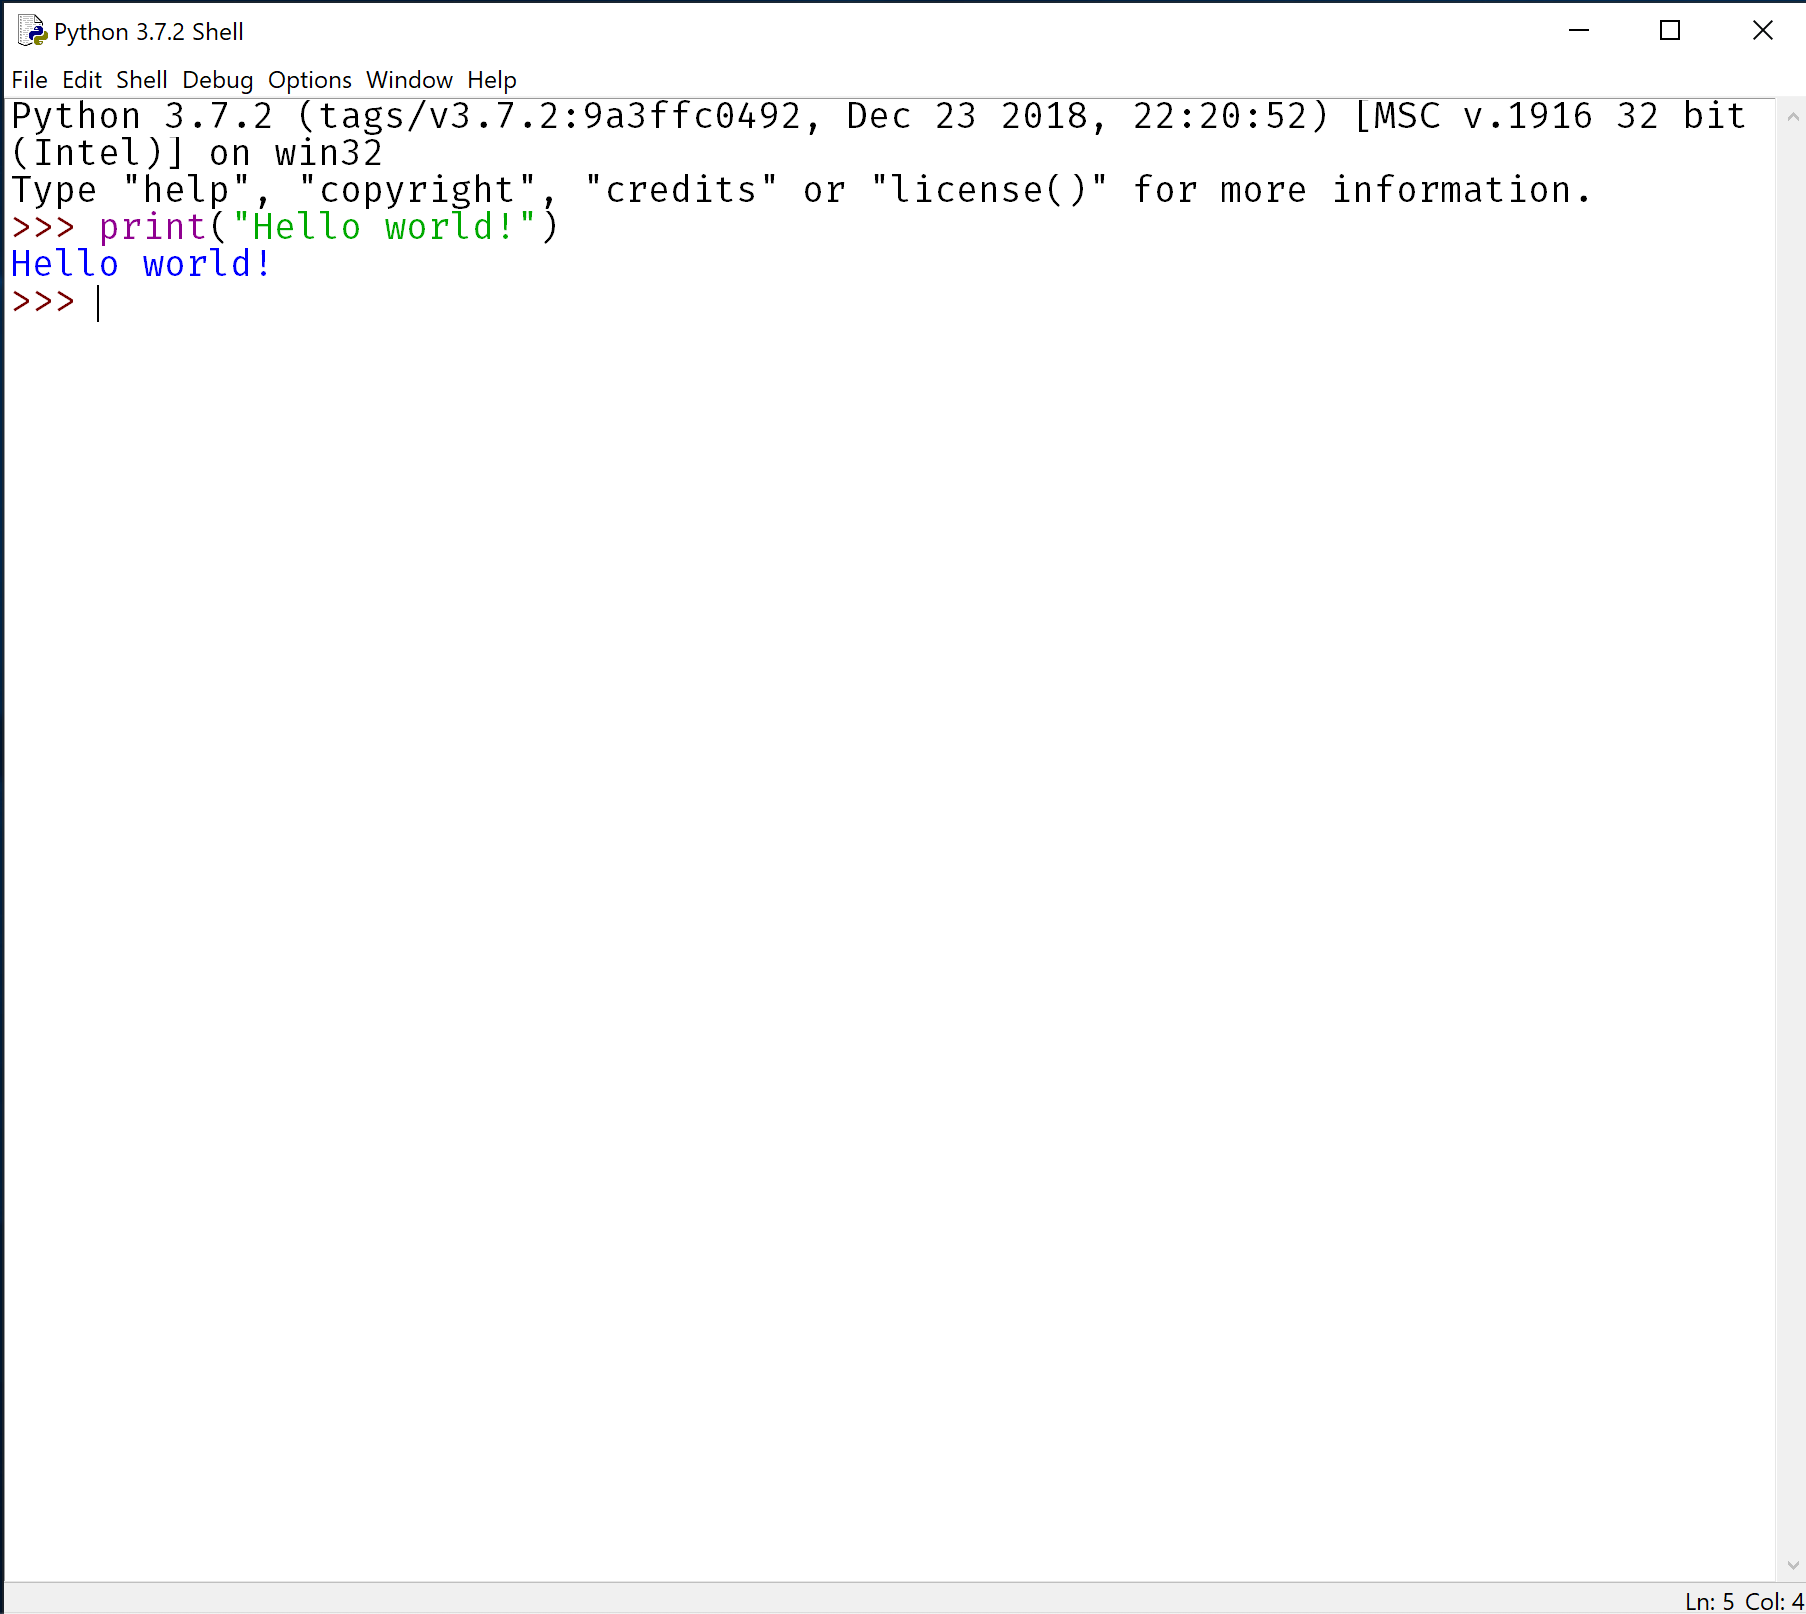
\includegraphics[scale=0.4]{screenshots/idlewin-hw}
\end{myfigure}

\subsection{Mac OS}

There are a couple of ways to install Python and IDLE for Mac OS, but the easiest way is probably the same as in Windows: to download the installation program from \url{https://www.python.org/downloads/} and install.

\subsection{Linux}

On my installation of Ubuntu Linux, I typed the following commands to install IDLE:

\begin{verbatim}
    $ sudo apt update
    $ sudo apt install idle
\end{verbatim}

You could also use the graphical software-installation tool to install IDLE.

Once it's installed, just type \verb-idle- at the command line prompt to open the program.  You should see something like the window in Figure \ref{fig:idlelinux} on Page \pageref{fig:idlelinux}.

\begin{myfigure}[label=fig:idlelinux]{IDLE Running on Ubuntu Linux}
    \centering
    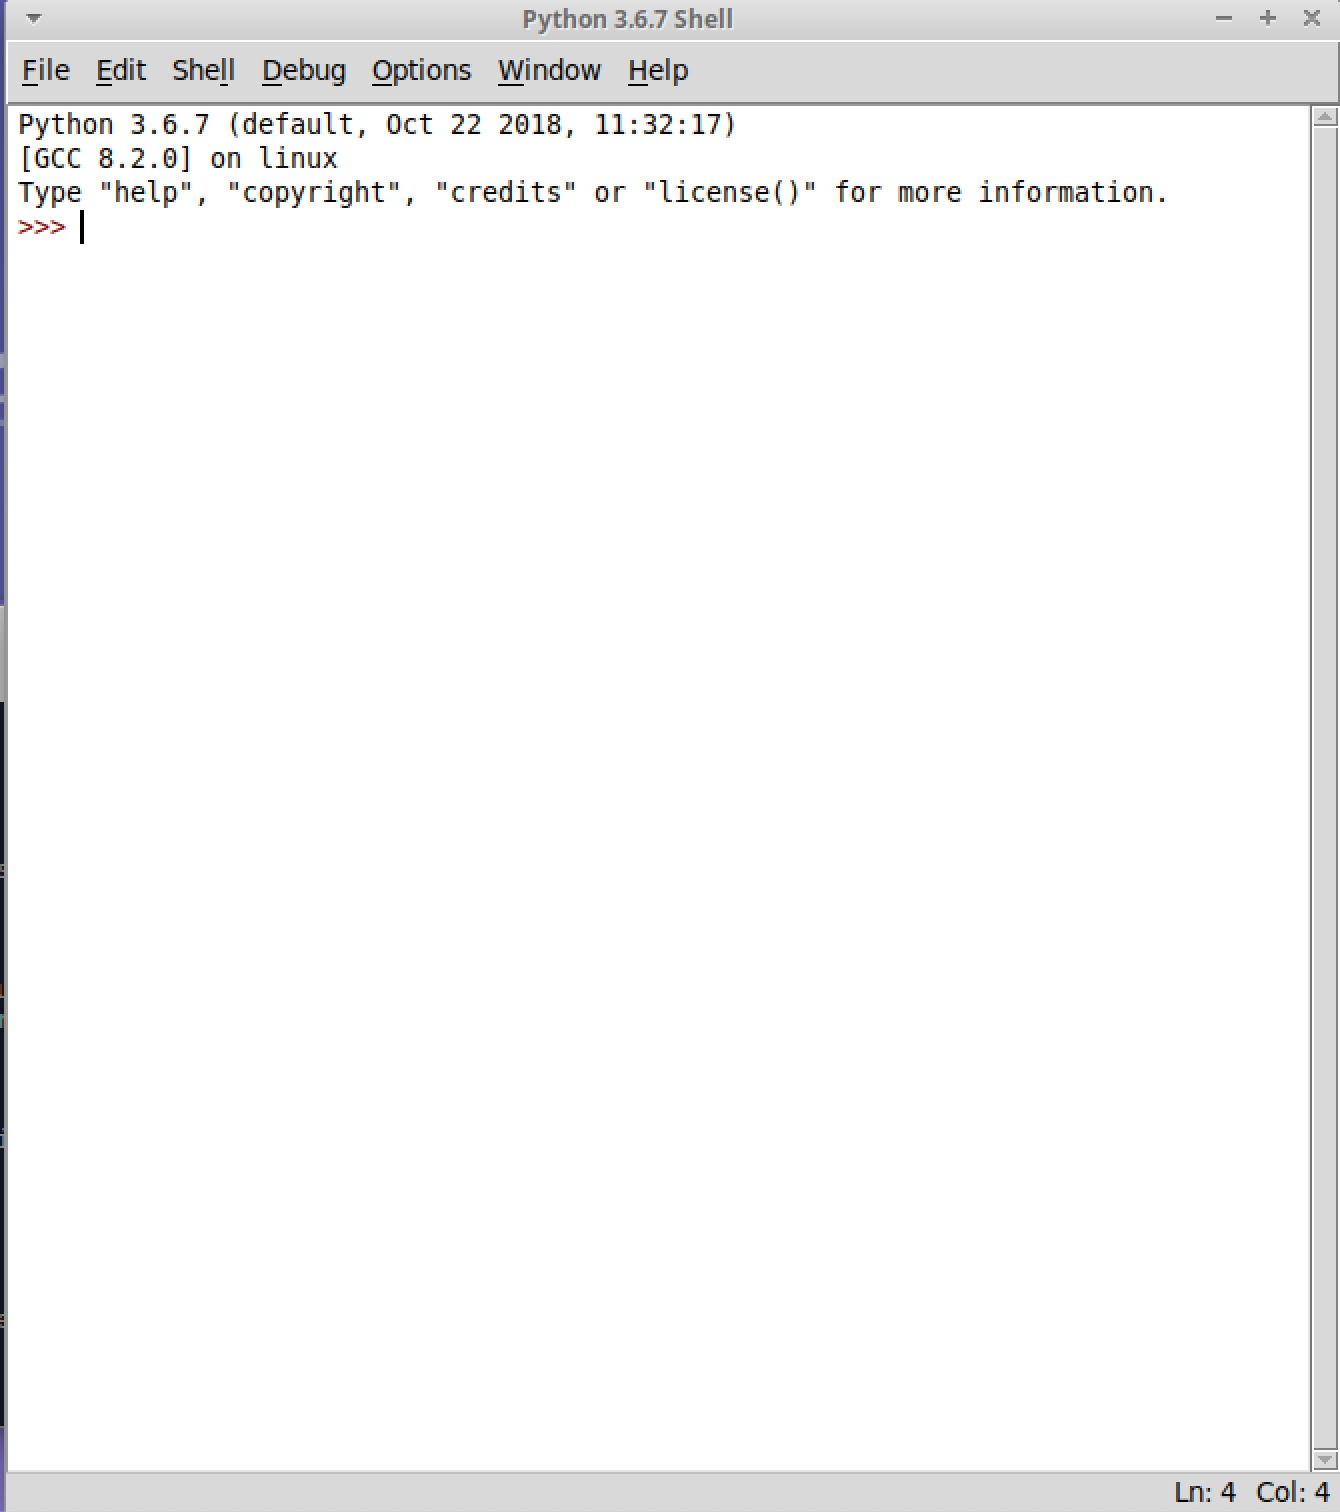
\includegraphics[scale=0.6]{screenshots/idlelinux.png}
\end{myfigure}

It is important that you see the phrase ``Python 3'' at the top of the screen (in this screenshot, it says ``Python 3.6.7'', and that's good).  If it says ``Python 2'' on the first line, then you are running an older version of IDLE -- and therefore an older version of Python -- and things won't work the way you expect.  If this is the case, try running \verb-idle3- instead of just \verb-idle-.  If that doesn't work, try to use \verb-apt- to install \verb-idle3-.